% !TeX root = ../main.tex
\section{Experimental Study: Five Paradigms at One Table}\label{sec:experiments}

The theory of Sections~\ref{sec:evaluation}--\ref{sec:rl} makes competing predictions. Rule-based play should be transparently exploitable; equilibrium play should be hard to exploit; learning should adapt to whatever field it faces. This section tests those predictions in silico: the five paradigms share one table in the engine described throughout the paper, and we measure win rates, aggression, and showdown statistics over $100{,}000$ hands of No-Limit Hold'em at blinds of 5/10 with 100-big-blind stacks.

\subsection{Setup and methodology}\label{sec:expsetup}

\paragraph{Agents.} All five agents run against the same engine API and the same shared abstraction (position class, street, card bucket, betting pattern; four abstract actions). The \emph{rule} agent instantiates Algorithm~\ref{alg:rule}. The \emph{Monte Carlo} agent estimates equity by $300$ simulated runouts per decision (the batch budget of Figure~\ref{fig:mcprecision}) and decides by pot odds with safety margins. The \emph{CFR (tabular)} agent plays the pooled average strategy of an external-sampling MCCFR self-play blueprint: $888{,}361$ iterations over $25$ minutes on the six-player abstract game, covering $72{,}741$ information-set instances that collapse to $13{,}873$ distinct pooled keys. The \emph{Deep CFR} agent plays the miniature advantage network of Section~\ref{sec:deepcfr} ($14 \to 32 \to 4$, reservoir of $60{,}000$ samples, validation correlation $0.44$). The \emph{RL} agent plays the tabular Q-function of Section~\ref{sec:rl} ($300{,}000$ episodes of self-play against a mixed pool, $6{,}585$ learned states, $\varepsilon = 0.02$ at play).

\paragraph{Design.} The study runs five blocks of $20{,}000$ hands. Each block seats the five paradigms plus a sixth \emph{shadow} seat duplicating one paradigm (block $k$ duplicates paradigm $k$), so that every paradigm faces every field composition; the shadow's results are excluded from all statistics, leaving exactly $100{,}000$ counted hands per paradigm. Seat assignment rotates by button-relative distance, so each paradigm occupies every position (button through big blind) uniformly. Stacks are reset to $100$ bb before every hand, which makes hands i.i.d.\ samples: per-paradigm win-rate estimates carry classical standard errors with no wealth-compounding correlation, and block effects can only enter through field composition, which the design varies deliberately. Deals are seeded and reproducible.

\paragraph{Engine correctness and fairness.} Three classes of invariant are asserted during play and three were verified offline before the study. In-play: chip conservation was asserted after every hand (total violated assertions over $10^{5}$ hands: \textbf{0}) and every agent action was validated against the legal-action set before application (illegal actions: \textbf{0}). Offline, in a prior audit: the dealer was verified card-by-card against an independent replication of the shuffle and deal logic ($0$ mismatches over $10^{5}$ hands); showdown winners were recomputed by a separate evaluator ($0$ disagreements); and side-pot awards were re-derived arithmetically ($0$ violations). Identical agents assigned to different seats showed no seat-dependent win-rate bias beyond multiple-testing noise. We therefore attribute observed differences to the agents.

\paragraph{Statistics.} Each paradigm's per-hand result $X$, measured in big blinds, has mean $\mu$ and variance $\sigma^{2}$ estimated from the $10^{5}$ samples; we report $100\hat\mu$ in bb/100 with standard error $100\sigma/\sqrt{10^{5}}$ (in bb/100) and $95\%$ confidence intervals. Pairwise differences of independent agents use the sphericity-free two-sample variance; with five agents there are $10$ pairwise comparisons, so isolated $z$-scores near $2$ should be read cautiously.

\subsection{Results}

Table~\ref{tab:results} reports the pooled statistics; Figure~\ref{fig:winrates} displays the win rates with confidence intervals, Figure~\ref{fig:styles} the style fingerprints, and Figure~\ref{fig:perblock} the per-block breakdown.

\begin{table}[!t]
\centering
\small
\renewcommand{\arraystretch}{1.32}
\setlength{\tabcolsep}{6.5pt}
\caption{Pooled results over $100{,}000$ hands per paradigm (five 20{,}000-hand blocks, rotating shadow seat; blinds 5/10; 100 bb stacks, reset every hand). Win rate in big blinds per 100 hands; $z = \hat\mu/\SE$. VPIP: hands voluntarily played; PFR: hands raised pre-flop; aggression: raise frequency over all decisions; SD: showdown frequency; SDW: showdown win rate.}
\label{tab:results}
\begin{tabular}{lrrrrrrrr}
\toprule
& \multicolumn{3}{c}{Win rate} & \multicolumn{3}{c}{Style fingerprint} & \multicolumn{2}{c}{Showdown} \\
\cmidrule(lr){2-4}\cmidrule(lr){5-7}\cmidrule(lr){8-9}
Agent & bb/100 & $\SE$ & $z$ & VPIP\,\% & PFR\,\% & Aggr\,\% & SD\,\% & SDW\,\% \\
\midrule
Deep CFR      & $+144.7$ & $21.0$ & $+6.9$  & $62.0$ & $58.7$ & $56.5$ & $37.2$ & $47.0$ \\
Rule-based    & $+79.3$  & $21.0$ & $+3.8$  & $60.9$ & $3.2$  & $10.8$ & $49.4$ & $44.2$ \\
RL (Q-learn)  & $-26.2$  & $5.2$  & $-5.1$  & $6.3$  & $4.7$  & $8.8$  & $2.5$  & $51.4$ \\
Monte Carlo   & $-51.9$  & $7.1$  & $-7.3$  & $25.2$ & $12.9$ & $15.6$ & $5.0$  & $59.2$ \\
CFR (tabular) & $-170.0$ & $17.5$ & $-9.7$  & $58.6$ & $46.6$ & $40.6$ & $25.7$ & $47.5$ \\
\bottomrule
\end{tabular}
\end{table}

\begin{figure}[htbp]
\centering
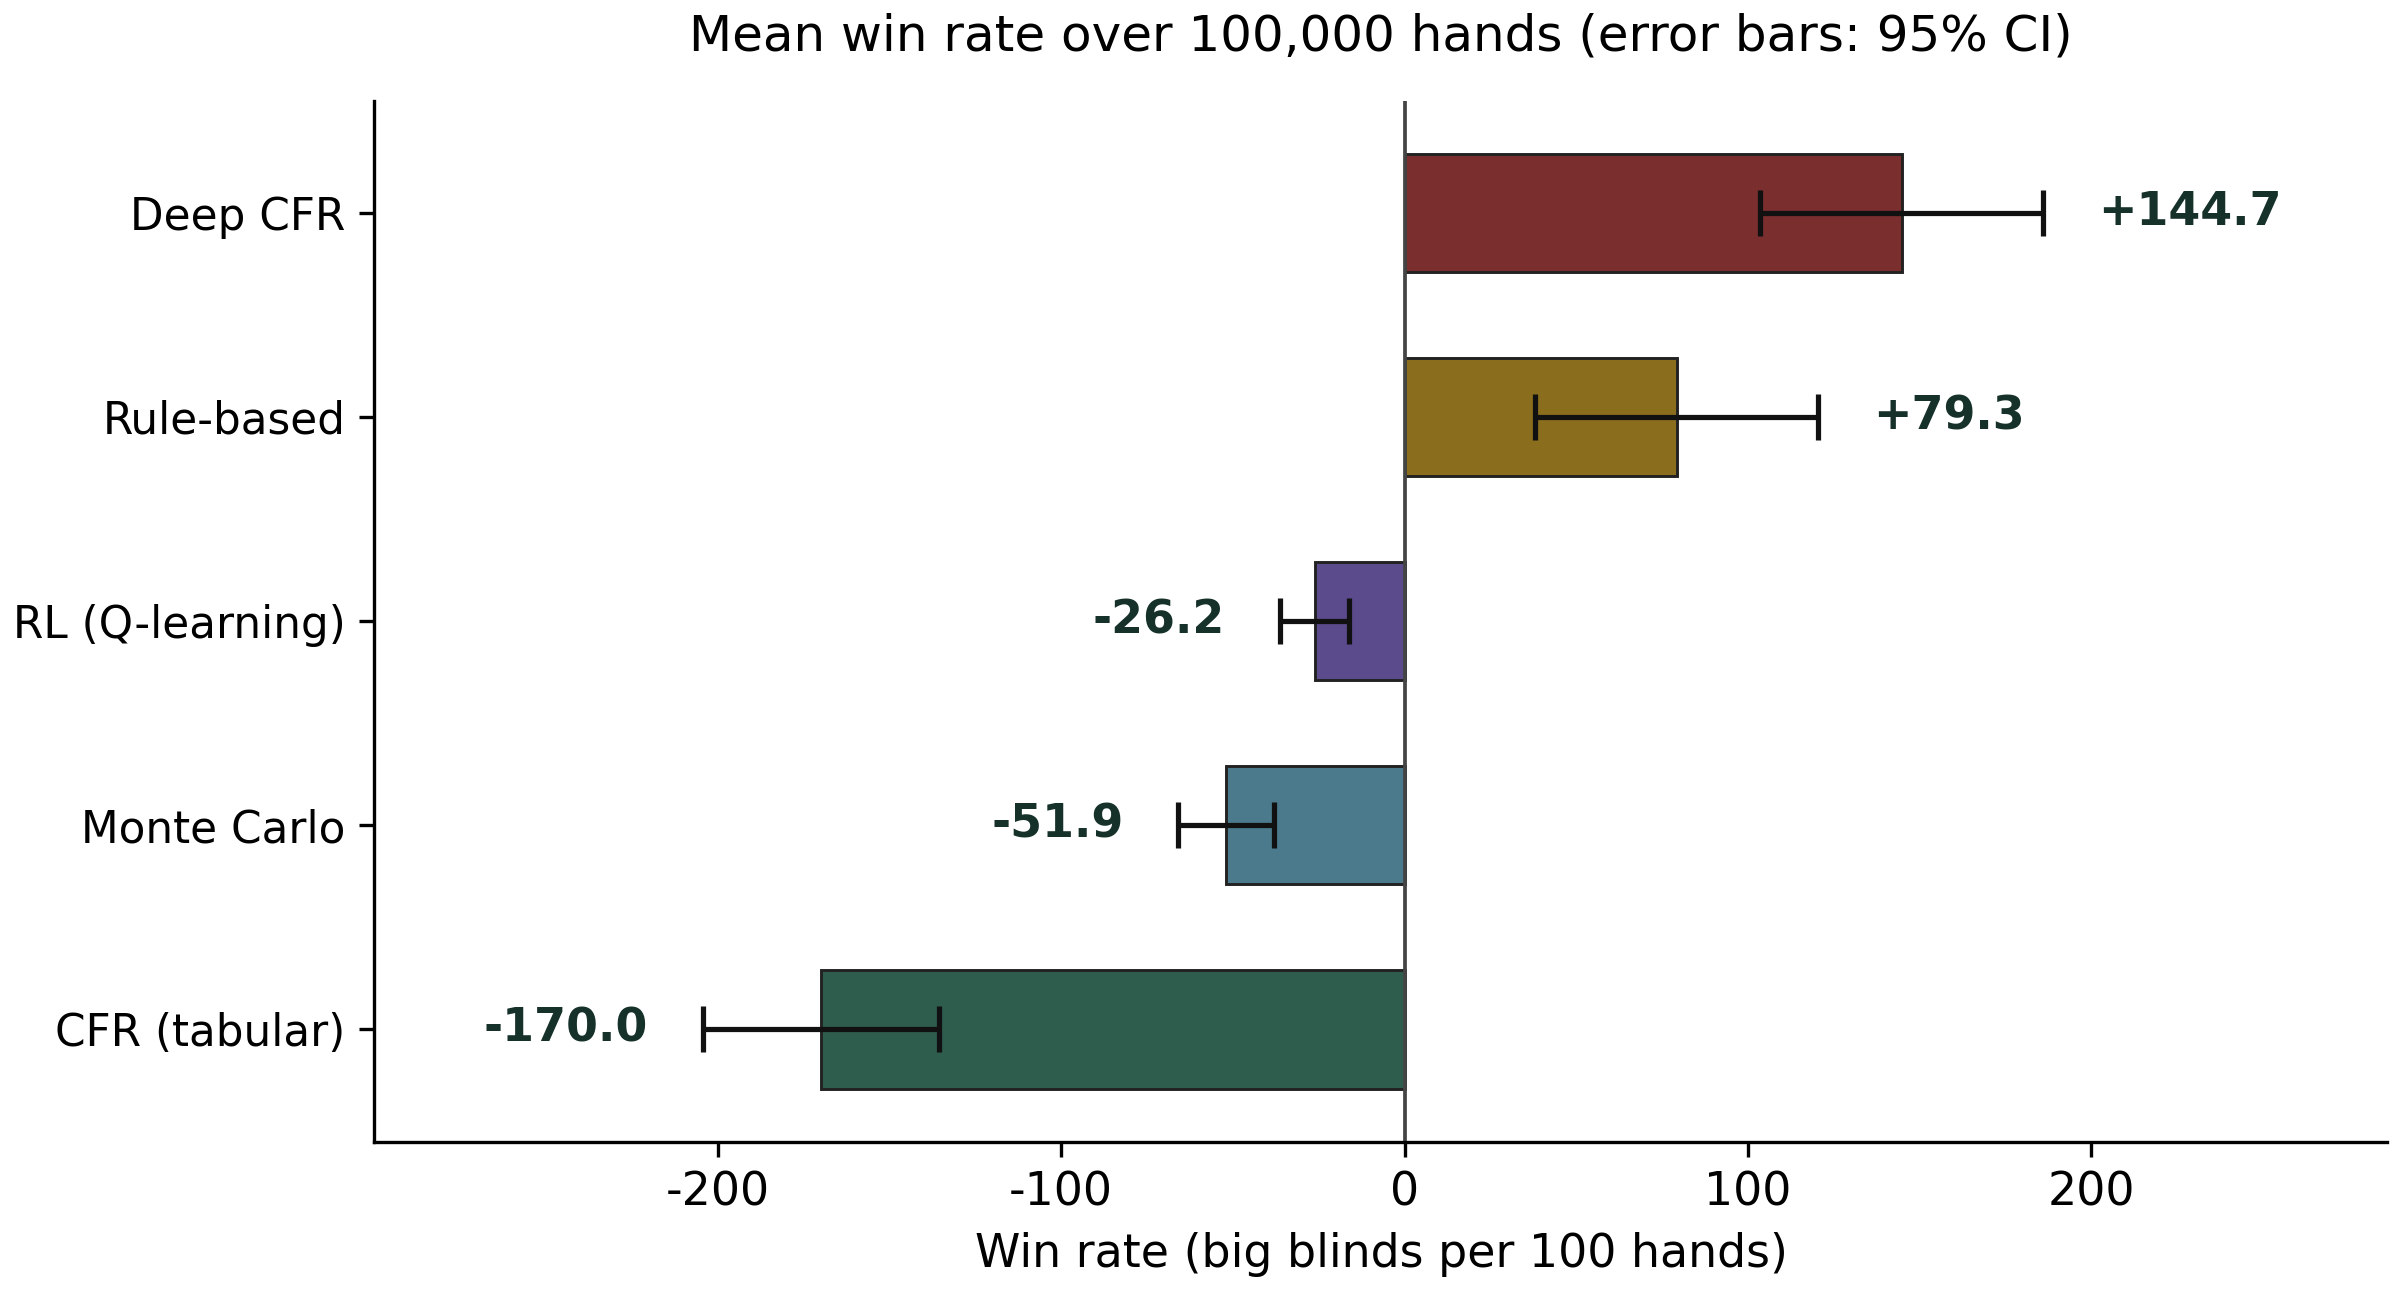
\includegraphics[width=0.94\textwidth]{figures/win_rates.png}
\caption{Mean win rate per paradigm over $100{,}000$ hands with $95\%$ confidence intervals. Every agent's win rate differs from zero significantly; the ordering is Deep CFR $>$ rule $>$ RL $>$ Monte Carlo $>$ tabular CFR, with the top and bottom agents separated by $11.5$ standard errors.}
\label{fig:winrates}
\end{figure}

Three headline facts emerge. First, \emph{every} win rate differs from zero significantly, and the pairwise separations are large: Deep CFR beats the tabular CFR agent by $314.7$\,bb/100 ($z = 11.5$) and beats the rule agent by $65.5$\,bb/100 ($z = 2.2$); the rule agent beats the tabular CFR agent by $249.3$\,bb/100 ($z = 9.1$). Second, the field is extraordinarily showdown-heavy: $64.0\%$ of hands reach showdown (against roughly $30\%$ in tight human six-max play), confirming that these agents neither fold enough nor steal enough. Third, per-hand volatility dwarfs the means---the standard deviation of a single hand's result ranges from $16$\,bb (RL) to $66$\,bb (rule, Deep CFR)---so the $10^{5}$-hand budget is what makes the ordering statistically decisive, precisely the regime \eqref{eq:handsneeded} anticipated.

\begin{figure}[htbp]
\centering
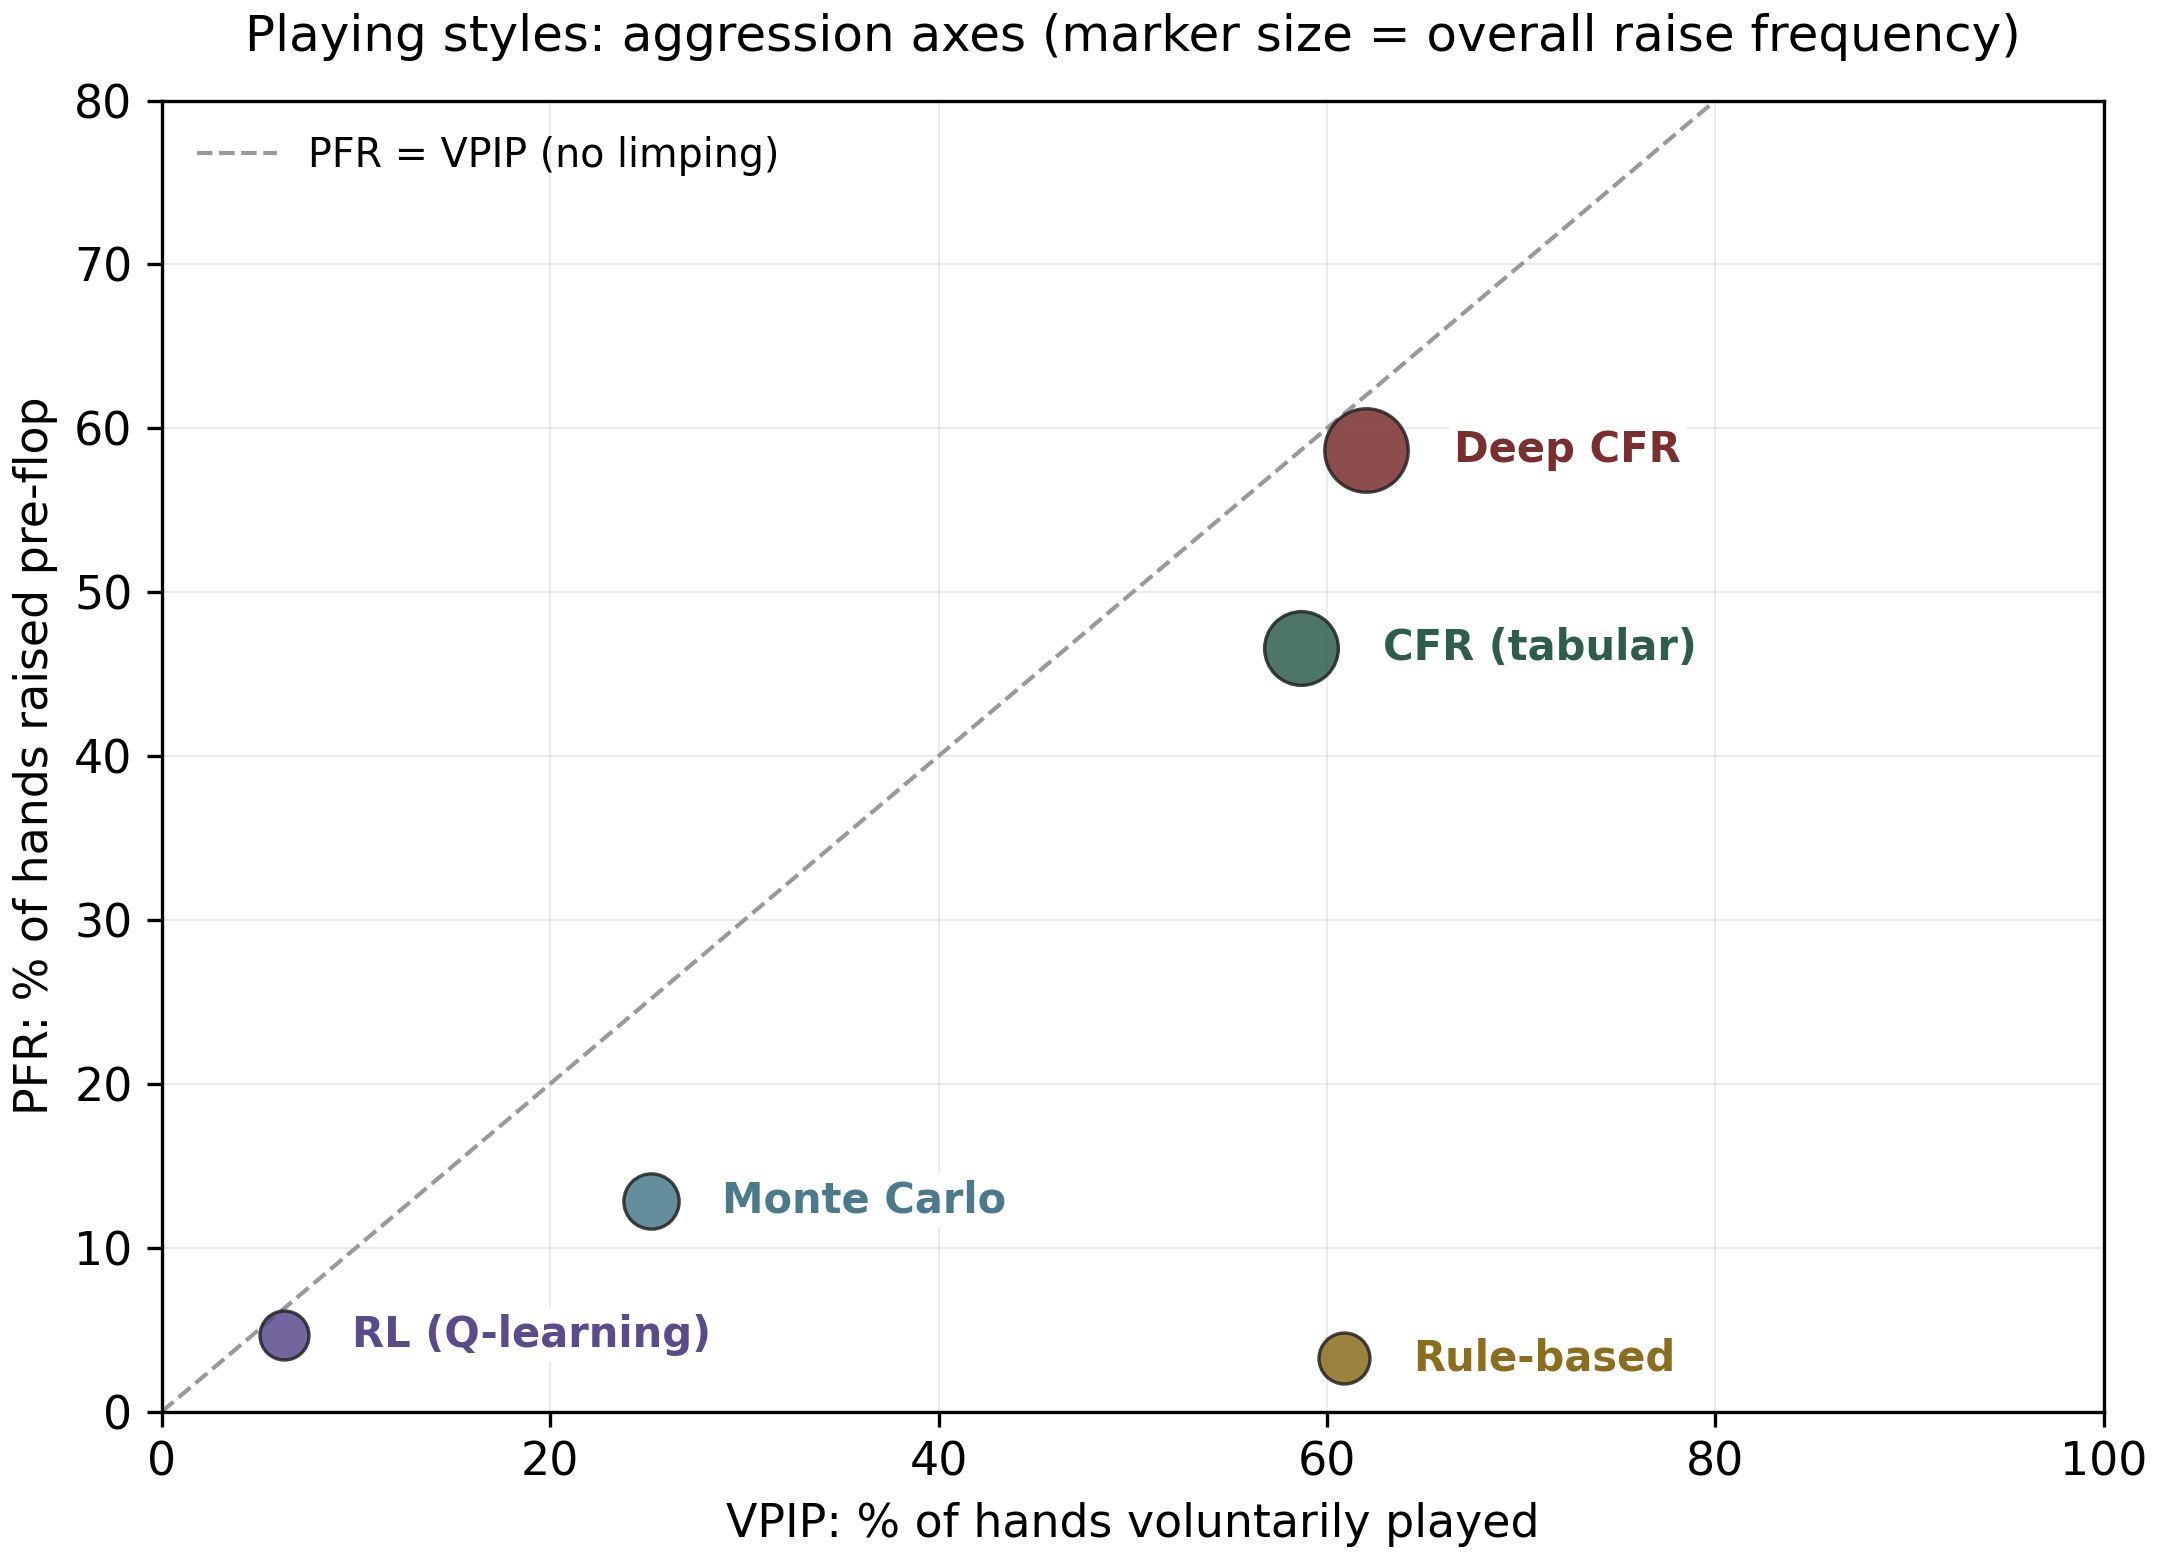
\includegraphics[width=0.86\textwidth]{figures/styles.png}
\caption{Style fingerprints in the VPIP--PFR plane (marker size proportional to overall raise frequency). The two CFR-family agents sit in the loose-aggressive quadrant with opposite fortunes; the rule agent is a loose-passive calling station; the RL agent learned an extreme nit profile; the Monte Carlo agent is tight and showdown-averse.}
\label{fig:styles}
\end{figure}

\subsection{Style analysis}

Figure~\ref{fig:styles} shows why the win-rate ordering is not a story about aggression alone. The two CFR-family agents occupy nearly the same loose-aggressive coordinates---CFR at (VPIP $58.6\%$, PFR $46.6\%$), Deep CFR at ($62.0\%$, $58.7\%$)---yet their win rates differ by $314.7$\,bb/100. The rule agent is their photographic negative: almost identical VPIP ($60.9\%$) but near-zero PFR ($3.2\%$), a textbook calling station that nonetheless wins $79.3$\,bb/100. The RL agent's learned policy is an extreme nit (VPIP $6.3\%$), folding everything except monsters---yet its showdown win rate when it does arrive ($51.4\%$) is second only to the Monte Carlo agent's $59.2\%$, and its losses are dominated by blind attrition. The Monte Carlo agent plays a tight-preflop, pot-odds-driven style that folds the flop to aggression (showdown frequency only $5.0\%$) and collects when it does continue ($59.2\%$ at showdown), a profile that is sound against balanced opponents and systematically wrong against a field that bets far too often.

\begin{figure}[htbp]
\centering
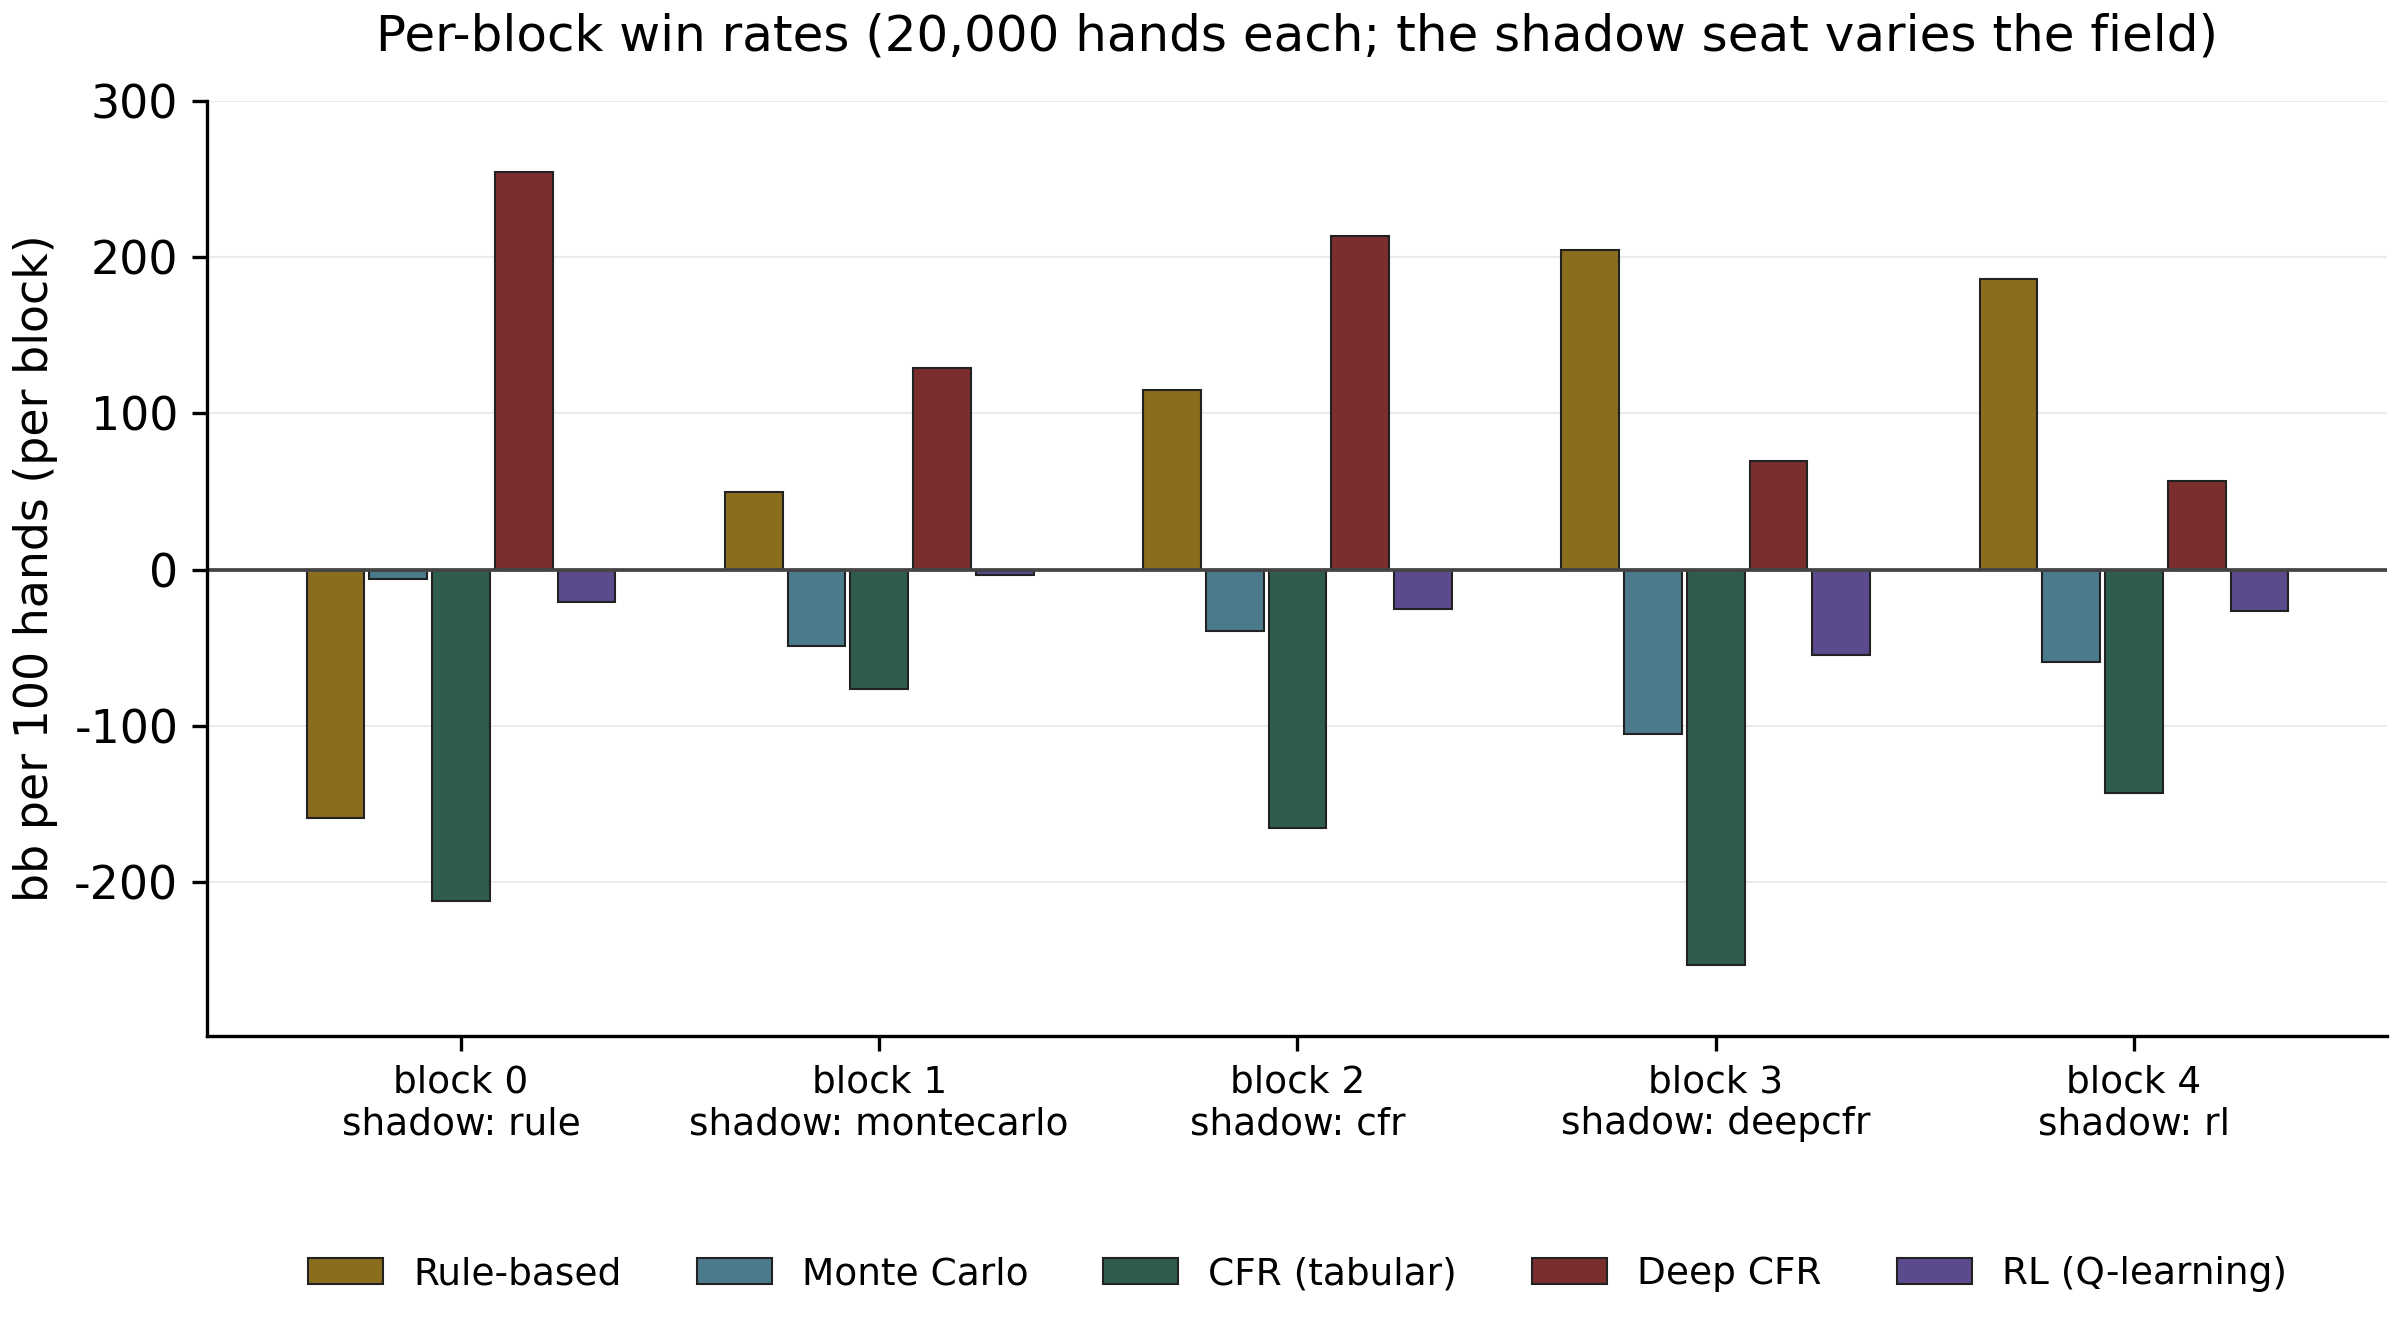
\includegraphics[width=0.94\textwidth]{figures/per_block.png}
\caption{Per-block win rates (20{,}000 hands per block). The shadow seat's identity (labelled below each block) changes the field composition; the ordering is largely stable across compositions, with Deep CFR the top or near-top earner everywhere and the tabular CFR agent losing in all five. The notable exception is the rule agent, whose result swings from $-159$\,bb/100 when the shadow duplicates itself to $+205$\,bb/100 when the shadow is the loose-aggressive Deep CFR---its calling-station style profits exactly when the extra opponent feeds it postflop calls---and the Monte Carlo / RL order flips in the block whose shadow duplicates the rule agent (with a second caller at the table, Monte Carlo's tight pot-odds play overtakes RL's blind-attrition losses).}
\label{fig:perblock}
\end{figure}

The per-block view (Figure~\ref{fig:perblock}) adds a robustness dimension: Deep CFR is the top or near-top earner in every field composition; the tabular CFR agent loses in all five; and the rule agent's two most profitable blocks are those whose shadow seats add either loose-aggressive opponents (Deep CFR, +$205$\,bb/100) or a second tight nit that surrenders blinds (RL, +$186$\,bb/100), while its worst block by far is the one whose shadow duplicates its own calling-station profile ($-159$\,bb/100).

\subsection{Interpretation: why did the equilibrium agent lose?}

The tabular CFR agent's $-170$\,bb/100 is the study's most instructive number, because it \emph{looks} like a refutation of Section~\ref{sec:cfr} and is in fact a layered confirmation of the theory's boundary conditions.

\emph{First, the multiplayer void.} CFR's guarantee---average strategy approaches an $\epsilon$-Nash equilibrium whose exploitability bound \eqref{eq:expl} protects the holder---is a two-player zero-sum statement (Theorem~\ref{thm:cfr} in conjunction with Section~\ref{sec:nash}). In a six-player game, regret minimisation against one's own self-play distribution converges toward a coarse correlated equilibrium-like object with \emph{no} safety property: Section~\ref{sec:nash}'s warning that multiplayer equilibrium is a robustness heuristic rather than an optimality certificate applies with full force to the blueprint we trained.

\emph{Second, the field calls.} Equilibrium aggression is priced for a rational responder: in Kuhn poker, the $1{:}3$ bluff--value ratio works because the opponent folds exactly often enough (Proposition~\ref{prop:kuhn}). This field does not fold---three of the five agents voluntarily play $58$--$62\%$ of hands and the table as a whole reaches showdown $64\%$ of the time---so bluffs at ``balanced'' frequencies become direct donations, and the blueprint's PFR of $46.6\%$ feeds pots to opponents who will pay to see rivers. The rule agent's profit is the mirror image of the same mispricing: a strategy that almost never bluffs and calls far too often is maximally punitive against an over-bluffing field, exactly as the Kuhn arithmetic predicts when the caller's folding rate deviates from equilibrium.

\emph{Third, the table is only partially converged.} Diagnostics on the trained blueprint quantify the practical gap between ``CFR in principle'' and ``this CFR run'': $18.7\%$ of the $13{,}873$ pooled strategy rows remain near-uniform (maximum action probability below $0.40$), and preflop rows---where most chips enter---are the least converged street (mean maximum probability $0.494$, against $0.64$--$0.68$ postflop). Whenever play reaches such a row, the agent acts near-uniformly over its legal actions: a sophisticated random player in exactly the spots that this field visits most. Months of compute close this gap in research systems; $25$ minutes does not.

\emph{Fourth, the sibling controls for the paradigm.} The decisive comparison is internal to the CFR family: same abstraction, same engine, same field, same training lineage---yet the tabular agent loses $170$\,bb/100 while the Deep CFR miniature wins $144.7$\,bb/100. The difference is not the learning principle but the \emph{representational fallback}: where the table has not been visited, it plays uniformly at random, whereas the advantage network outputs a smooth function of the state features and generalises to unvisited states. In a field this loose, coherence in the long tail of information sets is worth more than sharpness in the well-visited ones. We regard this as the study's cleanest lesson for practitioners: \emph{in small-budget settings, generalisation across information sets dominates table completeness.}

The RL agent's result completes the pattern. Its learned policy is a degenerate local optimum---folding all but $6\%$ of hands minimises variance against a training pool that included a random donor, and the terminal-only reward signal offered no gradient away from risk aversion. The policy was near-optimal \emph{against its pool} (training reward $+3.65$ chips per hand) and loses $-26.2$\,bb/100 against a different field: exploitation learned is field-specific, the guarantee asymmetry of Section~\ref{sec:nash} in miniature, produced by twenty seconds of self-play rather than by design.

\subsection{Threats to validity}

Four caveats bound the conclusions. (i) The study ranks \emph{implementations with these training budgets}, not paradigms: a months-scale blueprint, or a blueprint evaluated heads-up against a best responder, would occupy a different point in the space, and nothing here contradicts the exploitability guarantees that hold in two-player zero-sum settings. (ii) Field composition is endogenous: win rates are properties of the five-agent ecosystem, and adding one strong tight-aggressive agent would re-price every strategy in the table (the per-block swings of the rule agent make this visible). (iii) The shared abstraction, held fixed for comparability, is coarse (20 preflop and 10 postflop buckets, four abstract actions built from two raise sizes); all agents inherit its blind spots, and the Deep CFR agent's advantage is partly that its network interpolates across them. (iv) Statistical resolution, while sufficient for the headline separations (all $|z| \ge 2.2$; the top--bottom gap is $11.5\sigma$), cannot order agents within a few bb/100 of each other. With those boundaries stated, the study's summary is the one the theory foreshadowed: \emph{safety guarantees are field-independent but payoff-free against weak opponents; exploitation is field-relative and pays exactly as well as the field is exploitable; and representational generalisation decides who survives the long tail of states that training never reached.}
